% HEADERS
%%%%%%%%%%%%%%%%%%%%%%%%%%%%%%%%%%%%%%%%%%%%%%%%%%%%%%%%%%%%%%%%%%%%%%%%%%%%%%%%%%%%%%
\documentclass[11pt,a4paper]{report}
%\usepackage[italian]{babel}
\usepackage{graphicx}
\usepackage{wrapfig}
\usepackage{verbatim}
\usepackage{listings}
\usepackage{xcolor}
\usepackage{hyperref}
\usepackage{float}
\usepackage{titlesec}
\usepackage{nomencl}
\usepackage{amsmath}
\makenomenclature


\renewcommand{\vec}[1]{\mathbf{#1}}
\let\oldhat\hat
\renewcommand{\hat}[1]{\oldhat{\mathbf{#1}}}

\titleformat{\part}[display]
  {\Huge\bfseries}
  {}
  {0pt}
  {}

\titleformat{\chapter}[display]
 {\huge\bfseries}
 {}
 {0pt}
 {}

 \titleformat{\section}[display]
 {\Large\bfseries}
 {}
 {0pt}
 {\thesection\  \ }

\def\UrlBreaks{\do\/\do-}
\hypersetup{
    colorlinks=true,
    linkcolor=black,
    filecolor=magenta,
    urlcolor=cyan,
}
%\usepackage{url}
\definecolor{codegreen}{rgb}{0,0.6,0}
\definecolor{codegray}{rgb}{0.5,0.5,0.5}
\definecolor{codepurple}{rgb}{0.58,0,0.82}
\definecolor{backcolour}{rgb}{0.95,0.95,0.92}

\lstdefinestyle{mystyle}{
    backgroundcolor=\color{backcolour},
    commentstyle=\color{codegreen},
    keywordstyle=\color{magenta},
    numberstyle=\tiny\color{codegray},
    stringstyle=\color{codepurple},
    basicstyle=\ttfamily\footnotesize,
    breakatwhitespace=false,
    breaklines=true,
    captionpos=b,
    keepspaces=true,
    numbers=left,
    numbersep=5pt,
    showspaces=false,
    showstringspaces=false,
    showtabs=false,
    tabsize=2
}

\graphicspath{ {images/} }
\title{Orbital Mechanics Project}

\author{Marwan Alkady\\ Pedro Bossi N\'{u}\~{n}ez \\\ Demartini Davide\\ Iafrate Davide\\}
\date{\today}
%
%%%%%%%%%%%%%%%%%%%%%%%%%%%%%%%%%%%%%%%%%%%%%%%%%%%%%%%%%%%%%%%%%%%%%%%%%%%%%%%%%%%%%%
% ACTUAL DOCUMENT

\begin{document}

% FRONT COVER AND TABLE OF CONTENTS
%%%%%%%%%%%%%%%%%%%%%%%%%%%%%%%%%%%%%%%%%%%%%%%%%%%%%%%%%%%%%%%%%%%%%%%%%%%%%%%%%%%%%%
\begin{titlepage}
	\clearpage\thispagestyle{empty}
	\centering

%	Titles
%	Information about the University

   \centering 
\includegraphics[scale=0.7]{logo}

   \vspace{0.5cm}

	{\Huge\textbf{Politecnico di Milano} \\
Master of Science in\\ Space Engineering \\
		 \par}
		\vspace{3cm}
	{\Huge{Orbital Mechanics Project}} \\
	%\vspace{1cm}
	%{\large \textbf{xxxxx} \par}
	\vspace{3cm}
	{\huge Group 33\\}
	\vspace{0.4cm}
	{\LARGE Marwan Alkady 88888 - 88888888\\ Pedro Bossi N\'{u}\~{n}ez 887651 - 10561223\\ Davide Demartini 888657 - 10574461\\ Davide Iafrate 967709 - 10800009\\ \par}

%	Set the date
\vspace{1cm}
	{\Large A.Y. 2020-2021 \par}

	\pagebreak

\end{titlepage}

%\maketitle
\nomenclature{$a$}{semi-major axis}
\nomenclature{$e$}{eccentricity}
\nomenclature{$i$}{inclination}
\nomenclature{\omega}{periapsis anomaly}
\nomenclature{\Omega}{Right ascension of the ascending node}
\nomenclature{$f$}{true anomaly}

\printnomenclature
\tableofcontents

%%%%%%%%%%%%%%%%%%%%%%%%%%%%%%%%%%%%%%%%%%%%%%%%%%%%%%%%%%%%%%%%%%%%%%%%%%%%%%%%%%%%%%
% TEXT
%%%%%%%%%%%%%%%%%%%%%%%%%%%%%%%%%%%%%%%%%%%%%%%%%%%%%%%%%%%%%%%%%%%%%%%%%%%%%%%%%%%%%%
\part{Assignment 1: Interplanetary Explorer Mission}

\chapter{Mission requirements}
% table with:
% Departure Planet
% flyby planet
% arrival planet
% minimum departure and maximum arrival dates

\chapter{Mission analysis outputs}

\section{Design process}

\subsection{Initial choice for the time windows}

\subsection{Additional constraints considered}

\subsection{Transfer options exploration, analysis and comparison}

\subsection{Selection of the final solution}
% with plots and stuff

\section{Final solution}

\subsection{Heliocentric trajectory}
% Departure, flyby and arrival times.
% Plot of the heliocentric trajectory,together with the orbits of
% the three planets and their positions at departure, flyby and arrival.

\subsection{Powered gravity assist}
% Altitude of the closest approach.
% Time duration of the flyby (considering a finite SOI).
% Compare total flyby \Delta v with the cost of the manoeuvre \Delta v_{ga}
% Plot of the incoming and outcoming hyperbola arcs

\subsection{Cost of the mission}
%\Delta v_{dep}, \Delta v_{ga}, \Delta v_{arr}.

\part{Assignment 2: Planetary Explorer Mission}

\chapter{Mission requirements}
% table with:
% Central Planet
% Nominal operational orbit
% Orbit perturbations to be considered
% Ratio of satellite and Earth revolutions for the repeating ground track

\chapter{Mission analysis outputs}

\section{Nominal orbit}
%initial values and main characteristics

\section{Ground track}
% GT considering only J2 as perturbation and GT considering the assigned perturbation

\section{Orbit Perturbations}
In our model we included perturbations due to two effects:
\begin{itemize}
    \item \textbf{Second Zonal Harmonic \emph{J2}} \par Models the Earth Oblateness using the spherical geopotentials model, truncated to the second term.
    \item \textbf{Solar Radiation Pressure \emph{SRP}} \par A force given by the impact of momentum-carrying photons on the surfaces of the spacecraft. For this perturbation we have written a function that, based on the initial date 
\end{itemize}

These forces give an acceleration to the spacecraft so that the total acceleration it perceives in orbit is
\begin{equation}
    \vec{a} = - \frac{\mu_{\oplus}}{r^3}\vec{r} + \vec{a}_{SRP} + \vec{a}_{J2}
\end{equation}

\section{Orbit Propagation}
% In Cartesian coordinates and Keplerian elements through Gauss’ planetary equations,
%comparison of the propagation methods in terms of accuracy, computational time etc.
To propagate the orbit we used two different methods:
\begin{itemize}
    \item \textbf{Gauss Planetary Equations}
    \par
    \begin{align*}
        \frac{da}{dt}&=\frac{2a^2}{h}\Big(e\sin f \: a_r +\frac{p}{r}a_s\Big)\\[1]
        \frac{de}{dt}&=\frac{1}{h}\Big(p\sin(f) \: a_r+ \Big( (p+r)\cos f +re \Big) a_s\Big)\\[1]
        \frac{di}{dt} &= \frac{r\cos(f+\omega)}{h}a_w\\[1]
        \frac{d\Omega}{dt}&=\frac{r\sin (f+\omega) }{h \sin i}a_w\\[1]
        \frac{d\omega}{dt}&=\frac{1}{he} \Big( \cos f \; a_r + (p+r)\sin f \; a_s \Big ) - \frac{r\sin(f+\omega)\cos i}{h\sin i} a_w\\[1]
        \frac{df}{dt} &= \frac{h}{r^2} + \frac{1}{eh} \Big(p \cos f \; a_r - (p+r)\sin f \; a_s 
    \end{align*}

    \par
    We numerically integrate these equations with the ode113 solver, by using them to set the derivatives of the state.
    The reference frame for this equations is the RSW frame so $a_r, a_s, a_w$ are respectively the  radial, transversal and out-of-plane components. \cite{RSW_Curtis} \cite{RSW_Vallado} \cite{RSW_Battin}
    
    \item \textbf{Numeric integration of cartesian equations}
    This method consists in directly integrating the Cartesian equations of motion
    \begin{equation}
        \vec{\ddot{r}} = - \frac{\mu_{\oplus}}{r^3}\vec{r} + \sum{a_{p}}
    \end{equation}
    
\end{itemize}
There is a marked difference in the computational time between the two methods as the Gaussian elements propagation for a timespan of $50 T_{orbit}$ has a computation time $t_{GAUSS} = 5.4660*10^{-4} s$ that is much faster than the Cartesian $t_{CART} = 62.2 s$ one

\section{History of the Keplerian elements}
% plot the history of every keplerian element
%% UPDATE THE PLOTS WITH 1YEAR ONES
\begin{figure}[]
    \centering
    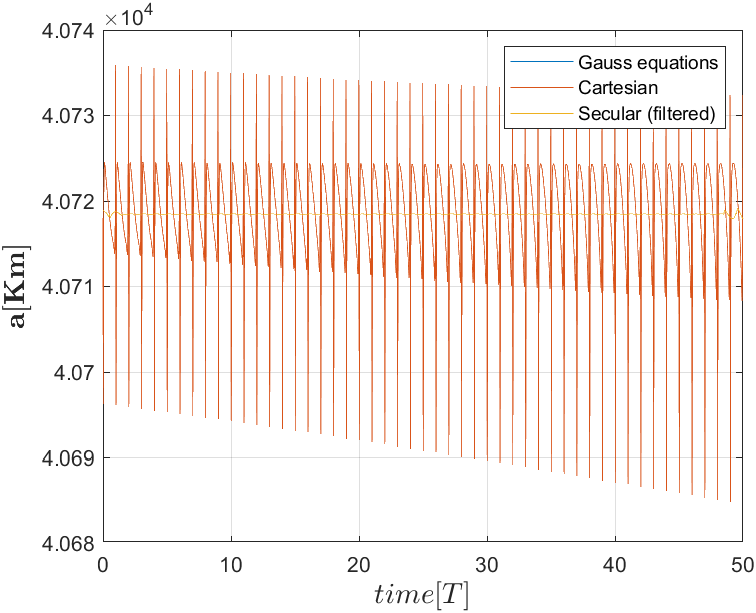
\includegraphics[semi-major axis evolution]{a.png}
    \caption{Evolution of the semi-major axis}
\end{figure}

\begin{figure}[]
    \centering
    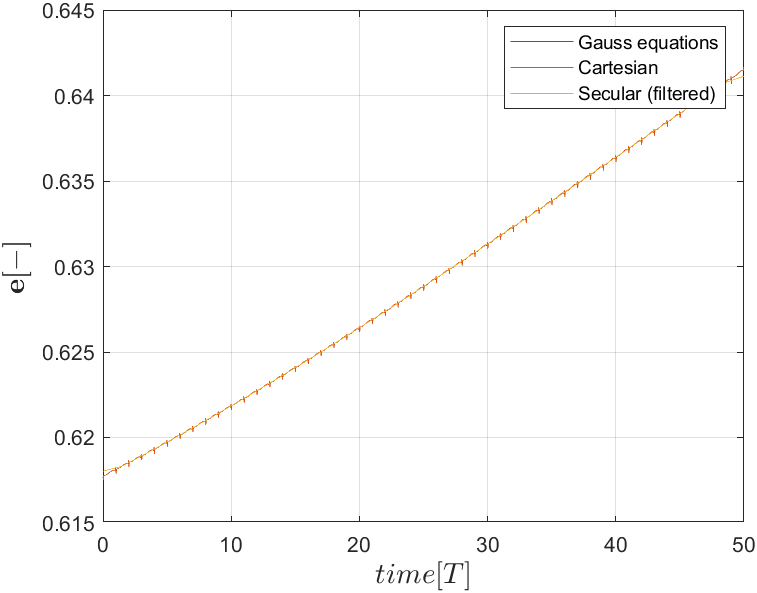
\includegraphics[eccentricity evolution]{e.png}
    \caption{Evolution of the eccentricity}
\end{figure}

\section{Orbit evolution representation}

\section{HF filtering}
%Maybe we can do it when we plot the history of the Keplerian elements
For the filtering we have used the simple \emph{movmean} function integrated in MATLAB which computes the average at each time instant between the current point and the neighboring ones with a cutoff period of $3T_{orbit}$.
\par We can see in the secular evolution that there is an increase in eccentricty due to the acceleration from the SRP being always in the same direction and the secular evolution has an oscillatory behaviour caused by Earth's revolution around the Sun. 

\section{Comparison with real data}

\subsection{Satellite selection}

\subsection{Comparison with our model}

\begin{thebibliography}{9}
\bibitem{RSW_Curtis} 
Curtis,H.D. 
\textit{Orbital mechanics for engineering students}. 
Butterworth-Heinemann , 2014. Chapter 12

\bibitem{RSW_Vallado} 
Vallado, D.A.
\textit{Fundamental of Astrodynamics and Applications, 4th
Ed}, Microcosm Press, 2013. Chapters 8 and 9

\bibitem{RSW_Battin} 
Battin, R,
\textit{An Introduction to the Mathematics and Methods of
Astrodynamics}, AIAA Education Series, 1999. Chapter 10
\end{thebibliography}

\end{document}
